\documentclass[preprint,12pt]{elsarticle}

\usepackage{amsmath}
\usepackage{newtxtext,newtxmath}
\usepackage{graphicx}
\usepackage{booktabs}
\usepackage{xcolor}
\usepackage{textcomp}
\usepackage[hidelinks]{hyperref}
\usepackage{lineno}
\linenumbers
\renewcommand{\topfraction}{0.9}
\renewcommand{\textfraction}{0.08}
\renewcommand{\floatpagefraction}{0.75}

\newcommand{\us}{\,\textmu s}
\newcommand{\um}{\,\textmu m}
\newcommand{\pending}[1]{\textcolor{red}{[PENDING: #1]}}

\journal{Aerospace Science and Technology}

\begin{document}

\begin{frontmatter}

\title{Response of a transverse-liquid-jet-anchored oblique detonation wave to jet interruption and pulsed injection}

\author{Yuvan Senthilkumar\corref{cor}}
\ead{yuvi.shen@outlook.com}
\cortext[cor]{Corresponding author.}
\address{Independent researcher}

\begin{abstract}
Transverse liquid jets can initiate and anchor liquid-fueled oblique detonation waves (ODWs), but only steady jets have been studied. This study computes how a liquid n-heptane ODW anchored by such a jet at a jet-inflow momentum ratio of J = 1 responds when the jet is switched off, switched back on, pulsed and throttled, with two-dimensional Eulerian--Lagrangian simulations validated against the steady-jet case. After the jet stops, the detonation survives. Its base holds for about 10\us\ and then retreats at about 0.12~mm/\textmu s, staying within 1~mm of the upstream end of the liquid layer the jet leaves on the wall, which slides downstream without losing mass; with that liquid removed, the base retreats 2.3 times sooner. A 1~mm jet leaves twice the liquid, and its layer and base move at half the speed. At 50\% duty, pulsing at 40 and 80~kHz keeps the steady-jet total-pressure recovery and burnt fuel with half the jet fuel, and 20~kHz does not, placing the critical frequency between 20 and 40~kHz. At 25\% duty and 80~kHz the base retreats as without a jet, although each off-time is shorter than the hold. At equal mean fuel, a half-width steady jet matches the pulsed jets in recovery, though its base drifts 2.2~mm downstream by the end of the run, and a jet throttled to J = 0.25 settles about 10~mm downstream. For a fixed injector, pulsing keeps the base at the jet at a fuel flow at which throttling does not.
\end{abstract}

\begin{keyword}
Oblique detonation wave \sep Transverse liquid jet \sep Pulsed injection \sep Liquid-fueled detonation \sep Detonation stabilization
\end{keyword}

\end{frontmatter}

\section*{Highlights}
\begin{itemize}
\item When the jet stops, the ODW survives but its base holds for only about 10\us.
\item Its base follows the wall liquid layer the jet leaves, not the jet itself.
\item Pulsing at 40--80 kHz and 50\% duty keeps steady-jet performance at half fuel.
\item At 25\% duty the base retreats as without a jet, despite off-times below the hold.
\item At equal fuel, a half-width steady jet matches pulsing in pressure recovery.
\end{itemize}

\section*{Nomenclature}
\begin{tabular}{@{}ll@{}}
$D$ & duty cycle, fraction of the period with the jet on (--)\\
$d_j$ & jet width (m)\\
$f$ & pulse frequency (Hz)\\
$f_\mathrm{cri}$ & critical pulse frequency (Hz)\\
$J$ & jet-inflow momentum ratio, $\rho_j u_j^2/(\rho_2 u_2^2)$ (--)\\
$p_0$ & total pressure (Pa)\\
$T_\mathrm{off}$ & off-time per pulse period, $(1-D)/f$ (s)\\
$u_j$ & jet velocity (m/s)\\
$v_r$ & retreat speed of the front base (m/s)\\
$x, y$ & coordinates along and normal to the wedge surface (m)\\
$\tau$ & hold time of the front base after the jet stops (s)\\
$\tau_\mathrm{lag}$ & delay between jet return and base recovery (s)\\
ODW, OSW & oblique detonation wave, oblique shock wave\\
ODWE & oblique detonation wave engine\\
\end{tabular}

\section{Introduction}

An oblique detonation wave (ODW) is an oblique shock wave (OSW) closely coupled with the heat release behind it. Burning a hypersonic airstream in a standing ODW gives a short combustor and a high thermal cycle efficiency, which makes the oblique detonation wave engine (ODWE) a candidate for hypersonic air-breathing propulsion \cite{Kailasanath2000,Jiang2023review,Rosato2021}. Standing ODWs have been established in shock-tunnel combustor experiments \cite{Zhang2022exp}, including with kerosene \cite{Han2023trip}. Holding one in a practical combustor still depends on two conditions: initiation must occur within the combustor length, and the wave must remain anchored as the inflow varies \cite{Jiang2023review,ZhangWen2025}.

Methods for controlling ODW initiation fall into three groups. Geometric methods alter the compression surface: stepped wedges \cite{Qin2018modified}, on-wedge trips \cite{Han2023trip} and bumps \cite{Liu2026bump}, and wedges whose angle is adjusted in response to the flow \cite{Sun2023unsteady}. Energy deposition heats the mixture locally, by laser hot spots \cite{Xin2024laser} or plasma; Jiang et al. \cite{Jiang2025energy} showed that pulsed deposition sustains an on-wedge ODW at 2.3--6.5\% of the average power that continuous deposition needs. They also showed that it does so only above a critical pulse frequency $f_\mathrm{cri}$, derived from the arrival times of the waves that successive pulses produce; $f_\mathrm{cri}$ fell from about 25 to 8.5~kHz as the pulse energy increased. Fluidic methods inject a jet into the flow: hot jets \cite{Wang2022hotjet,Li2020hotjet,Qin2020coflow}, cold transverse jets \cite{Han2024jet,ZhangJiang2023jet} and jet--wedge combinations \cite{Yao2023jetwedge}. Of these, only the sweeping jet of Fan et al. \cite{Fan2024sweeping} is unsteady; according to Ref.~\cite{Wang2026ast}, its periodically redirected gas jet shortened the initiation length by 25\% relative to a wedge without a jet and kept it steadier than a steady jet as the jet pressure varies.

Liquid hydrocarbon fuels make both initiation and anchoring harder. Droplets must break up and evaporate before the gas can react, and evaporation cools the mixture behind the shock. Ren et al. showed that wedge-induced ODWs in two-phase kerosene--air mixtures initiate and stabilize differently from gaseous ones \cite{Ren2018jfm}, and examined their dependence on the equivalence ratio \cite{Ren2019pci}. In partially pre-vaporized n-heptane sprays, the initiation length first increases and then decreases with droplet diameter, with unsteady propagation behind the front \cite{Teng2023droplet,Tian2024jfm}. In a pre-injection ODWE combustor at Mach~9 and 30~km, a pure n-heptane spray does not form an ODW at all \cite{Wang2025cnf}.

Wang, Hu and Zhang \cite{Wang2026ast} showed on an open 27\textdegree\ wedge that a transverse n-heptane jet initiates an ODW in an n-heptane spray that otherwise fails to ignite. At J $\le$ 0.3 the jet mainly enriches the near-wall mixture and the ODW forms downstream, whereas at J $\ge$ 0.4 the jet acts as an obstacle whose OSW initiates detonation directly. In a confined combustor, the same group found a finite window of J inside which a steady jet keeps the ODW confined, including under sinusoidal inlet-pressure forcing at 4 and 8~kHz \cite{Wang2026confined}. There the wave system follows the forcing through bounded mode transitions, with triple-point excursions of 3--5~mm at a forcing amplitude of 0.5.

In all of this work on liquid jets, the jet is steady. Switching the jet raises three questions: how long the detonation stays anchored once the jet stops, what holds it during that time, and how fast the jet must be pulsed to keep it held. The first two have not been measured for any jet-anchored ODW. The third has been answered for pulsed energy deposition \cite{Jiang2025energy} but not for a pulsed fuel jet, which leaves liquid in the flow after each pulse. A search of the English and Chinese literature in October 2026, including the 2025 review of ODW initiation in confined combustors \cite{ZhangWen2025}, found no study of an interrupted or pulsed liquid jet for ODW control. The closest results are the hysteresis of ODWs under wedge-angle changes \cite{Liu2018hysteresis}, which shows that the final wave depends on its history, and the sweeping gas jet \cite{Fan2024sweeping}.

The present study takes the open-wedge J = 1 case of Ref.~\cite{Wang2026ast} as its baseline, reproduces it, and then switches and pulses the jet. It measures the hold time of the front base after the jet stops, isolates the part of it due to the residual liquid, and relates the base position to the motion of that liquid. It measures the retreat that follows and the lag before the base recovers when the jet returns, varies the jet width, and tests how far these quantities account for the response to pulsing at 20--80~kHz and at 50 and 25\% duty. Finally, it compares the pulsed jets with steady jets that use the same mean fuel, either through a narrower slot or through a throttled jet of the same width. The rest of the paper is organized as follows. Section~\ref{sec:method} describes the numerical method, the reduced domain used for the parametric runs, and the diagnostics. Section~\ref{sec:results} presents the anchored baseline, the response to jet interruption, the pulsed-jet results and their performance, and the comparison at equal fuel. Section~\ref{sec:conclusions} summarizes the conclusions.

\section{Computational methodology}\label{sec:method}

\subsection{Governing equations and sub-models}

The gas phase obeys the two-dimensional, multi-component, compressible Navier--Stokes equations with source terms for interphase exchange,
\begin{align}
\frac{\partial \rho}{\partial t} + \nabla\cdot(\rho\mathbf{u}) &= S_m, \label{eq:mass}\\
\frac{\partial (\rho\mathbf{u})}{\partial t} + \nabla\cdot(\mathbf{u}\rho\mathbf{u}) + \nabla p - \nabla\cdot\boldsymbol{\tau} &= \mathbf{S}_F, \\
\frac{\partial (\rho E)}{\partial t} + \nabla\cdot[\mathbf{u}(\rho E + p)] + \nabla\cdot\mathbf{q} - \nabla\cdot(\boldsymbol{\tau}\cdot\mathbf{u}) &= S_e, \\
\frac{\partial (\rho Y_i)}{\partial t} + \nabla\cdot(\mathbf{u}\rho Y_i) - \nabla\cdot(\rho D_i \nabla Y_i) &= \dot\omega_i + S_{Y,i}, \quad i = 1,\dots,n_s-1, \label{eq:species}
\end{align}
closed by the ideal-gas law, Sutherland's law for viscosity and a unity Lewis number. Chemistry follows the 44-species, 112-reaction skeletal n-heptane mechanism of Liu et al. \cite{Liu2004mech}, as in Ref.~\cite{Wang2026ast}. The liquid is tracked as Lagrangian parcels with drag, heat transfer and evaporation. The sub-models follow the baseline authors' published solver case \cite{Wang2024breakup}: Pilch--Erdman breakup \cite{Pilch1987}, Ranz--Marshall heat transfer \cite{Ranz1952}, and a sphere drag law with $C_d = 0.424$ above a droplet Reynolds number of 1000. The two phases are coupled through particle-source-in-cell sources \cite{Crowe1977}. Equations (\ref{eq:mass})--(\ref{eq:species}) and the droplet equations are those of Ref.~\cite{Wang2026ast} and are not repeated here.

The equations are solved with detonationFoam \cite{Sun2023detonationfoam} (two-phase branch, on OpenFOAM-8), using Kurganov--Noelle--Petrova fluxes \cite{Kurganov2001}, limited-linear reconstruction, first-order Euler time stepping and a Courant number of 0.3, as in Ref.~\cite{Wang2026ast}. Two sub-models differ from that reference. Evaporation uses OpenFOAM's boiling-aware model in place of the Abramzon--Sirignano model \cite{Abramzon1989}, which OpenFOAM-8 does not provide. The droplet--wall interaction, which Ref.~\cite{Wang2026ast} does not state, is a rebound. The wall is a slip wall, and no turbulence model is used.

\subsection{Configuration and conditions}

The configuration is the open-wedge case of Ref.~\cite{Wang2026ast} (Fig.~\ref{fig:schematic}). A single 27\textdegree\ wedge stands in for the inlet of an ODWE flying at Mach~9 and 30~km. The domain is aligned with the wedge surface, with $x$ along the wall from the leading edge and $y$ normal to it. Table~\ref{tab:conditions} lists the inflow and jet conditions. The inflow carries n-heptane droplets at stoichiometric loading. A liquid n-heptane jet issues normally from the wall at $x$ = 50~mm. The jet-inflow momentum ratio is
\begin{equation}
J = \frac{\rho_j u_j^2}{\rho_2 u_2^2},
\end{equation}
where subscript 2 denotes the state behind the wedge OSW. J = 1 corresponds to $u_j$ = 60.83~m/s. The jet's droplet sizes follow a Rosin--Rammler distribution with a mean of 10\um. Ref.~\cite{Wang2026ast} gives only the mean; the spread ($n$ = 3, 1--30\um) is chosen here. Parcels are injected with equal mass, so the distribution applies by mass, and the number-mean droplet diameter is smaller than 10\um. The case is two-dimensional with a depth of 2~mm, and all mass flows below are per 2~mm of depth.

Ref.~\cite{Wang2026ast} states the jet width and velocity but no mass flow; here the jet carries $\rho_l u_j d_j$ per unit depth, that of a solid liquid slot. On the 0.2~mm grid the 0.5~mm jet is represented by two wall faces, 0.4~mm wide, carrying that mass flow at the stated velocity, so that the mass and momentum per unit depth are those of the 0.5~mm jet; the momentum flux per unit area is then 1.25 times the nominal value. J is quoted by velocity, as in Ref.~\cite{Wang2026ast}. The continuous jet injects 41.4~g/s, against 9.7~g/s of fuel carried by the inflow spray across the whole domain boundary.

\begin{table}[tbp]
\centering
\caption{Inflow and jet conditions, from Ref.~\cite{Wang2026ast}.}\label{tab:conditions}
\begin{tabular}{@{}ll@{}}
\toprule
Inflow pressure, temperature, velocity & 28.55~kPa, 697.0~K, 2535.0~m/s\\
Inflow droplets & n-C$_7$H$_{16}$, 10\um, 300~K, stoichiometric\\
Wedge angle & 27\textdegree\\
Jet position, width & $x$ = 50~mm, 0.5~mm\\
Jet fluid, velocity at J = 1 & liquid n-C$_7$H$_{16}$, 60.83~m/s\\
Jet droplets & Rosin--Rammler, mean 10\um\\
\bottomrule
\end{tabular}
\end{table}

\begin{figure}[tbp]
\centering
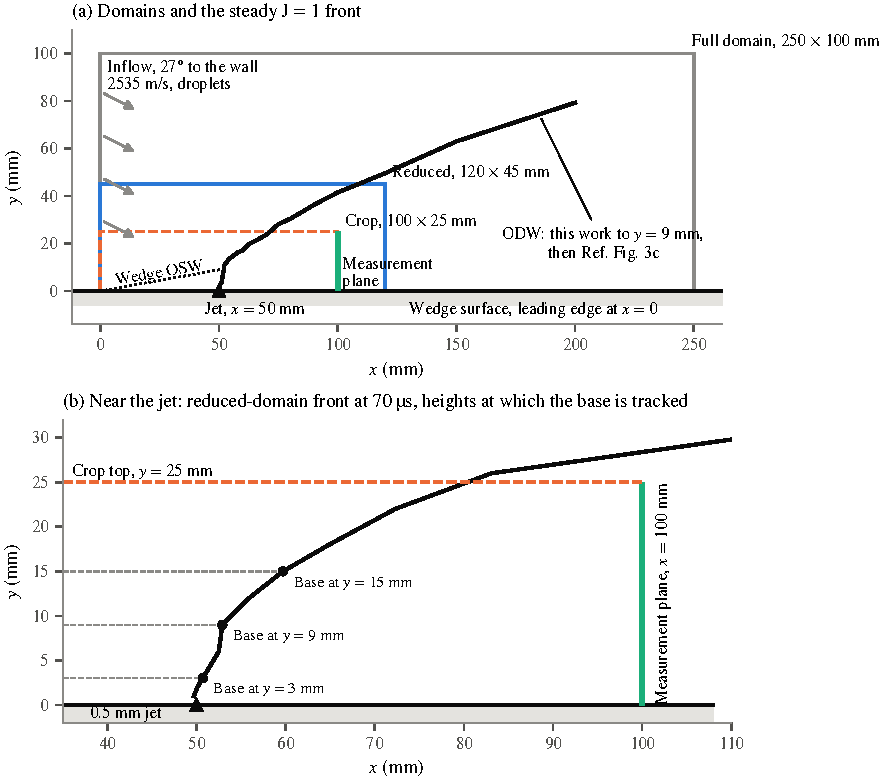
\includegraphics[width=\linewidth]{figures/fig_schematic.pdf}
\caption{Computational configuration, in the frame aligned with the wedge surface. (a) The full domain follows Ref.~\cite{Wang2026ast}; the jet is switched and pulsed in the reduced domain, whose front near the jet matches the full domain (Section~\ref{sec:reduced}), and the grid and follow-up tests use the crop. The front is the computed steady J = 1 front at 100\us\ up to $y$ = 9~mm and the front of Ref.~\cite{Wang2026ast}, Fig.~3c, above; the wedge OSW is drawn to the computed shock height at $x$ = 52~mm. (b) The front of the reduced domain at 70\us\ near the jet, with the base positions at the heights at which the base is reported. Performance is measured on the plane $x$ = 100~mm, $y <$ 25~mm.}\label{fig:schematic}
\end{figure}

\subsection{Validation}\label{sec:validation}

The thermodynamic data of the mechanism, as read by the solver, give $c_p$ and $h$ identical to Cantera's between 300 and 2500~K, and a constant-pressure ignition at 1400~K, 2.8~bar and $\phi$ = 1 reaches 1700~K at 84.8\us, against 86.1\us\ for the same criterion in Cantera. For the premixed n-heptane ODWs of Guo et al. \cite{Guo2023pci} on a 30\textdegree\ wedge, the computed post-shock temperatures are 1454 and 1603~K at $\phi$ = 1 and 0.2, against 1452 and 1601~K reported, and the simulated initiation lengths, defined as in Ref.~\cite{Guo2023pci} by the heat-release peak along the wall, are 21.7~mm at $\phi$ = 1, with an abrupt transition (19.8~mm reported), and 4.1~mm at $\phi$ = 0.2, with a smooth transition (3.47~mm reported).

For the open-wedge configuration, three cases of Ref.~\cite{Wang2026ast} were rerun. With pre-vaporized fuel and no jet, the wall temperature is 1481, 2345 and 2990~K at $x$ = 10, 55 and 75~mm, against 1452, 2295 and 2928~K reported. With the droplet inflow and no jet, the near-wall gas stays at 1110--1206~K over 60\us\ with no ignition, as reported. With the jet at J = 1 on the full domain, the jet-induced ODW forms at the jet and the main ODW develops downstream, the mechanism reported for J $\ge$ 0.4. Figure~\ref{fig:validation} compares the front height. At $x$ = 52--70~mm the front lies 0.5--1.8~mm below that of Ref.~\cite{Wang2026ast} and rose by at most 0.2~mm between 90 and 100\us; at $x$ = 75--120~mm it lies 3--7~mm below and was still rising by 0.2--1.0~mm per 10\us\ at the end of the run. Beyond $x$ = 150~mm the main ODW was still developing when the run ended (49.5 against 63.0~mm at $x$ = 150~mm at 90\us), because the inflow droplets were lost at the start of that run and its effective development time is shorter than the published one; this region does not affect the near-jet front, and the parametric runs do not include it. Near the jet, where the results of this study lie, the front agrees with Ref.~\cite{Wang2026ast} to within 2~mm, of which about 1~mm is the uncertainty in reading the published figure. Candidate causes of the remaining offset are inputs Ref.~\cite{Wang2026ast} does not state: the droplet size spread of the jet, the droplet--wall model and the 0.4~mm jet patch.

\begin{figure}[tbp]
\centering
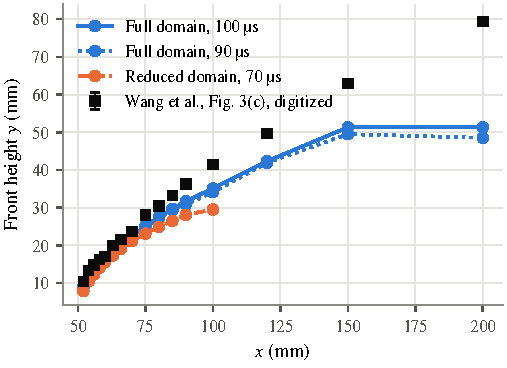
\includegraphics[width=0.62\linewidth]{figures/fig_validation.pdf}
\caption{Front height of the J = 1 case against $x$ (top of the region above 1900~K), compared with Ref.~\cite{Wang2026ast} Fig.~3(c) at 100\us, whose values are read to about $\pm$1~mm (error bars): full domain at 90 and 100\us, reduced domain at 70\us. Beyond $x$ = 120~mm the main ODW of the full-domain run was still developing when the run ended.}\label{fig:validation}
\end{figure}

\subsection{Reduced domain and branching protocol}\label{sec:reduced}

The full domain (6.25 $\times$ 10$^5$ cells) is too costly for a parametric study made of runs of 70--130\us. The jet experiments are therefore run in a reduced domain of 120 $\times$ 45~mm (1.35 $\times$ 10$^5$ cells) with the same grid, boundary conditions and jet, started from the uniform freestream. A smaller domain (90 $\times$ 35~mm) gave the same front up to $y$ = 26~mm to within 0.4~mm at equal times, but its end cuts the front at $y$ = 30--34~mm, so the larger one is used. In the reduced domain the front at $y$ = 1--4~mm holds the full-domain position ($x$ = 49.9--51.5~mm) from 35\us\ onward. At 70\us\ the near-wall gas upstream of the jet is at 1156~K, 2.74~atm and 2081~m/s (full domain: 1134~K, 2.75~atm, 2083~m/s), and the jet shock at $y$ = 3~mm sits at $x$ = 50.9~mm in both. On the measurement plane defined below, total-pressure recovery and burnt fuel agree with the full domain at equal times (0.123 and 0.121 against 0.123 and 0.115 at 95 and 100\us).

Every jet setting starts from the same reduced-domain state at 70\us\ by restarting from its saved fields, so that the droplet cloud is carried over and all branches share the same liquid inventory at switch time. The continuous-jet run, continued to 145\us, is the reference. Its front at $y$ = 3~mm moves by less than 0.2~mm over 70--145\us. Its performance is not stationary, however. The liquid within 30~mm of the jet grows from 3.5~mg at 80\us\ to 6.2~mg at 140\us, about 44~g/s against the 41~g/s the jet injects: all of the jet liquid stays near the wall, and some freestream liquid collects with it. The reference recovery falls from 0.137 at 70\us\ to 0.113 at 145\us. All comparisons are therefore made at equal times, never against a fixed reference value.

\subsection{Jet interruption and pulsing}

The jet is switched as a square wave of frequency $f$ and duty cycle $D$, beginning with an on-phase at 70\us. The off-time per period is $T_\mathrm{off} = (1-D)/f$, and the mean jet fuel is $D$ times that of the continuous jet. Table~\ref{tab:cases} lists the cases. Two steady jets carry the same mean fuel as the 50\% pulses: one at half the velocity (J = 0.25, below the J $\ge$ 0.4 that Ref.~\cite{Wang2026ast} found for direct initiation) and one at half the width (a single 0.2~mm face at J = 1, with the same momentum flux per unit area as the full jet). The second is one cell wide and is injected by a cone injector on that face rather than across the patch, so its comparison carries that caveat. To vary the jet width, a 1~mm jet at J = 1 was run in the crop: five wall faces carrying $\rho_l u_j d_j$, so that its momentum flux per unit area is the nominal value, against 1.25 times nominal for the 0.5~mm jet on its 0.4~mm patch.

\begin{table}[tbp]
\centering
\footnotesize
\caption{Cases. Those above the rule branch from the continuous J = 1 reduced-domain run at 70\us; those below run in the crop of Section~\ref{sec:grid}. Mean jet fuel is relative to the continuous 0.5~mm jet.}\label{tab:cases}
\begin{tabular}{@{}lllll@{}}
\toprule
Case & Jet & $T_\mathrm{off}$ & Jet fuel & Run (\textmu s)\\
\midrule
Reference & continuous, J = 1 & -- & 100\% & 70--145\\
Jet off & off & -- & 0 & 70--200\\
Jet off, dry & off, jet liquid removed at 70\us & -- & 0 & 70--90\\
Jet on again & off, on again at 95\us & -- & -- & 95--130\\
80~kHz & $D$ = 0.5 & 6.25\us & 50\% & 70--145\\
40~kHz & $D$ = 0.5 & 12.5\us & 50\% & 70--145\\
20~kHz & $D$ = 0.5 & 25\us & 50\% & 70--145\\
Half velocity & continuous, J = 0.25 & -- & 50\% & 70--200\\
Half width & continuous, J = 1, one face & -- & 50\% & 70--145\\
\midrule
\multicolumn{5}{@{}l}{\textit{Crop, branched at 50\us}}\\
Jet off (two grids) & off & -- & 0 & 50--90\\
80~kHz, $D$ = 0.25 & $D$ = 0.25 & 9.4\us & 25\% & 50--90\\
1~mm jet & continuous, J = 1 & -- & 200\% & 0--50\\
1~mm jet off & off & -- & 0 & 50--80\\
\bottomrule
\end{tabular}
\end{table}

\subsection{Diagnostics}

\textit{Front base.} Along lines of constant $y$, the detonation front is taken as the first pressure rise of at least 30\% of the largest rise on the line that has CO$_2$ mass fraction above 0.02 within 0.8~mm behind it. The search windows are fixed in length, not in cells. Requiring burnt gas behind the rise rejects the bow shock of a weakened jet and downstream compressions, which a largest-rise criterion mistook for the front, with errors of up to 14~mm for weak or absent jets. The base position is reported at $y$ = 3~mm. At $y$ = 1~mm the jet bow shock and the base lie within a few cells of each other, so that height is not used.

\textit{Performance.} Total-pressure recovery and burnt fuel are measured on the plane $x$ = 100~mm, $y <$ 25~mm, which the stream processed by the jet crosses. Recovery is the mass-flux-weighted total pressure across the plane divided by that entering the domain. The total pressure of each cell is the isentropic stagnation pressure of the gas phase at frozen composition over all 44 species; it matches Cantera to 0.005\% for the freestream, burnt gas, fuel-rich burnt gas and cold heptane-rich gas. Retaining only the major species would overestimate the recovery by 0.004--0.012, because C$_2$H$_2$, H$_2$ and C$_2$H$_4$ make up 7\% of the mass of the fuel-rich burnt gas near the wall. Burnt fuel is the fuel-equivalent carbon in CO$_2$ and CO crossing the plane. The domain outflow is not used, because evaporative cooling of the unshocked spray raises the gas-phase total pressure there above the inflow value. Values are averaged over five saves 5\us\ apart, which span one period at 40~kHz and two at 80~kHz at evenly spaced phases.

The save-to-save scatter of the reference about its trend is $\pm$0.002 in recovery and $\pm$0.04~g/s in burnt fuel, so differences below 0.003 and 0.08~g/s are not resolved. This is the scatter within one run. The run-to-run scatter from the random injection positions was not measured. Recovery on the plane responds to a change at the jet only after 35--50\us: over 95--115\us\ the jet-off case differs from the reference by only twice the noise floor, whereas over 120--130\us\ the difference is 0.036. Only windows from 120\us\ onward are used to compare cases.

\subsection{Grid independence}\label{sec:grid}

Ref.~\cite{Wang2026ast} found the 0.15 and 0.2~mm grids to agree along a streamline 20~mm from the wall, and used 0.2~mm. Because the present results rest on a time scale (the hold time after switch-off) rather than on a steady profile, that check is repeated for the transient. A 100 $\times$ 25~mm crop of the reduced domain around the jet was run at 0.2 and 0.15~mm to 50\us, and switched off at 50\us. On the 0.15~mm grid the jet patch is three faces (0.45~mm) wide, so its momentum flux per unit area is 11\% lower than on the 0.2~mm grid at the same mass and momentum per unit depth. Over 40\us\ after switch-off, the base at $y$ = 3~mm on the two grids agrees within 0.1~mm at every 5\us\ save: both hold for about 10\us, retreat at 0.13~mm/\textmu s and stand at 54.7 and 54.8~mm after 40\us, from 50.7~mm (Fig.~\ref{fig:grid}). The crop agrees with the reduced domain within 0.2~mm over the same interval. At $y$ = 9~mm the grids agree within 0.3~mm. The tracker's search windows are fixed in physical length, so the diagnostic itself does not change with the grid. The hold time and retreat speed are therefore independent of the grid at the 0.2~mm resolution used here, and of the crop, which is used for the 25\% duty and 1~mm jet cases below.

\begin{figure}[tbp]
\centering
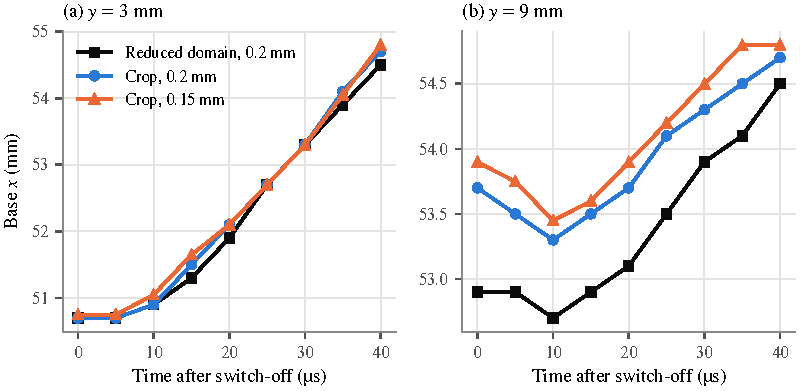
\includegraphics[width=\linewidth]{figures/fig_grid.pdf}
\caption{Grid and domain independence of the response to switch-off: base position at (a) $y$ = 3~mm and (b) $y$ = 9~mm against time after the jet stops, in the reduced domain (0.2~mm, switched off at 70\us) and in the crop on the 0.2 and 0.15~mm grids (switched off at 50\us).}\label{fig:grid}
\end{figure}

\section{Results and discussion}\label{sec:results}

\subsection{The jet-anchored front}\label{sec:baseline}

Figure~\ref{fig:baseline} shows the near-jet region of the reference at 70\us. The values in this subsection are taken from the full-domain case at 85--95\us, which the reduced domain matches near the jet (Section~\ref{sec:reduced}). The gas approaching the jet along the wall is at 1134~K and 2.75~atm with an n-heptane vapour mass fraction of 0.093. Its constant-pressure ignition delay is 2385\us, against 24\us\ to convect from the leading edge to the jet, so this gas cannot ignite on its own within the domain. The jet raises an OSW whose foot, 1--4~mm from the wall, holds at $x$ = 49.7--51.5~mm with a pressure ratio of 6.5--8.5. Behind it the frozen state is 1920--2150~K and the ignition delay 0.13--0.44\us. Behind the jet-induced OSW the ignition delay is four orders of magnitude shorter than in the gas approaching the jet, so the base sits at the foot of that shock.

Downstream of the jet, the jet liquid forms a wall layer that is cold and fuel-rich. Between $x$ = 50 and 65~mm, a subsonic pocket moves at 157~m/s. Beyond it, a layer with an n-heptane vapour mass fraction of 0.45, at 748~K and nearly free of oxygen (O$_2$ 0.013), extends along the wall to $x$ = 182~mm. Within 30~mm of the jet the domain holds 4.1~mg of liquid in about 68,000 parcels with a median diameter of 5.2\um. That is all the liquid the jet has injected; the jet liquid breaks up but barely evaporates or moves downstream.

In the reduced-domain reference at 80\us, the droplets within $x$ = 50--80~mm and $y <$ 3~mm are at 382~K and the gas around them at 410~K, with an n-heptane vapour mass fraction of 0.59; 15\us\ after the jet is switched off they are at 399 and 418~K. At the latter state the Spalding mass-transfer number is 0.59, and the $d^2$-law lifetime of a 5\um\ droplet is about 230\us. The pocket evaporates more slowly still: between 5 and 25\us\ after switch-off its liquid stays at 3.09--3.14~mg while breakup reduces the mass-weighted diameter from 5.6 to 4.2\um, so evaporation removes less than 2\% in 20\us, a depletion time above 1~ms. Ref.~\cite{Wang2026ast} estimates about 0.5~ms for a 10\um\ droplet in the 697~K inflow, about 125\us\ for 5\um\ by the $d^2$ law. The pocket is surrounded by its own cool vapour (410--418~K, vapour mass fraction 0.59), which is consistent with its slow evaporation. Ref.~\cite{Wang2026ast} reports the same cooling along its near-wall streamline (about 700~K behind the jet) but not the colder inner pocket. Averaged over $x$ = 49.5--80~mm and $y <$ 3~mm, the liquid occupies 2.5\% of the volume. It is concentrated in the 194 wall cells that hold parcels, however, where it is about 30\% of the volume and 20 times the gas mass. This is far outside the dilute-spray assumption behind point-particle models; the pocket is in effect a wall film represented by parcels. Because the pocket barely evaporates, what changes after the jet stops is not its mass but its position (Section~\ref{sec:off}), and that motion is governed by the drag of a dense liquid layer, which the point-particle model represents least reliably.

\begin{figure}[tbp]
\centering
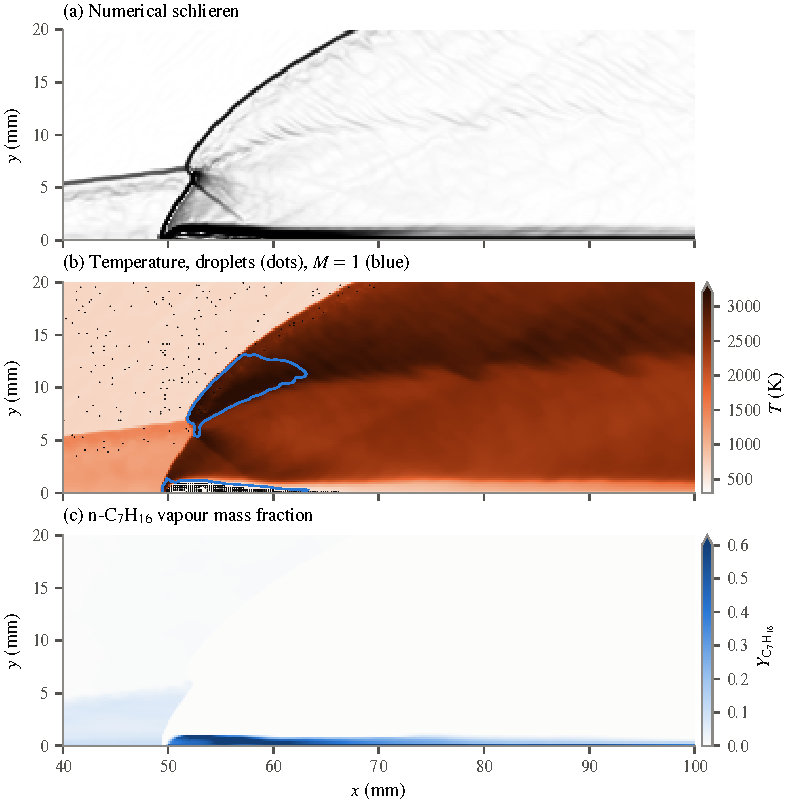
\includegraphics[width=\linewidth]{figures/fig_baseline.pdf}
\caption{Near-jet structure of the J = 1 reference at 70\us. (a) Numerical schlieren, $\exp(-15|\nabla\rho|/|\nabla\rho|_{99.5})$. (b) Temperature with jet and freestream droplets (dots, 6000 drawn at random); the blue contour is $M$ = 1 and bounds the subsonic regions. (c) n-C$_7$H$_{16}$ vapour mass fraction. The jet-induced OSW anchors the detonation at $x \approx$ 50~mm; behind the jet, the liquid forms a cold, fuel-rich wall layer.}\label{fig:baseline}
\end{figure}

\subsection{Response to jet interruption}\label{sec:off}

Figure~\ref{fig:off} shows the base position after the jet is switched off at 70\us. The detonation does not fail. For about 10\us\ the base stays where it was. It then retreats downstream at 0.12--0.13~mm/\textmu s at $y$ = 3~mm ($x$ = 50.9~mm at 10\us, 56.7~mm at 60\us), while the front above $y$ = 9~mm moves much less: at $y$ = 15~mm it stays at $x$ = 59.1--60.1~mm for 35\us. By 35\us\ after switch-off the lowest 6~mm of the front have straightened into one front at $x \approx$ 54~mm (Fig.~\ref{fig:offsnap}). This is consistent with the loss of the jet-induced OSW at the base, after which the base drifts to where the remaining compression still ignites the mixture.

The hold comes mainly from the residual liquid. When all jet liquid is removed at the moment of switch-off, the base retreats at once and reaches $x$ = 54~mm 2.3 times sooner than when the liquid is left in place (Fig.~\ref{fig:off}). With the liquid left in place, the pocket persists after the jet stops (2.9~mg at 105\us, 35\us\ after switch-off) and still obstructs the near-wall flow. A second test, in which droplets reaching the wall are removed rather than reflected, left the pocket almost unchanged (2.95 against 3.11~mg at 80\us) and the front unchanged. It also altered the near-wall inflow upstream of the jet (1171 against 1143~K), so it does not isolate the wall model, and the hold time may still depend on how a real wall film behaves.

The base follows the position of the liquid, while the liquid mass hardly changes. Figure~\ref{fig:edge} follows the liquid within $y <$ 3~mm downstream of the jet in the crop, where the response to switch-off matches the reduced domain (Section~\ref{sec:grid}). After switch-off its mass stays at 2.2~mg for 30\us, but the layer slides downstream as a whole: the point below which 25\% of the liquid lies moves from $x$ = 50.7 to 54.5~mm between 50 and 80\us\ (0.14~mm/\textmu s over 55--80\us), and the liquid within 3~mm of the jet drains to zero in 25\us. The base at $y$ = 3~mm stays 0--1.0~mm upstream of that 25\% point at every save through 25\us\ after switch-off, with the jet on as well as off. Only once the layer has largely left the region, 30--40\us\ after switch-off, does the base fall behind it, by up to 2.4~mm. The hold is the time before the upstream end of the layer starts to move, and the retreat speed is the speed at which the gas drags the layer downstream; the pocket's subsonic core moves at a similar 0.16~mm/\textmu s with the jet on (Section~\ref{sec:baseline}). This correspondence is observed in three runs (Sections~\ref{sec:model} and \ref{sec:duty}); the causal evidence is the dry run above.

\begin{figure}[tbp]
\centering
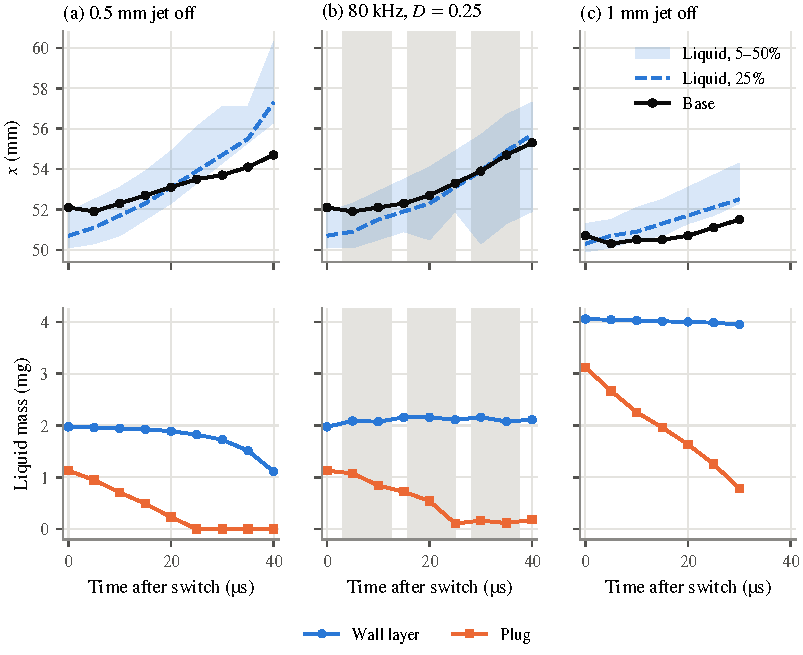
\includegraphics[width=\linewidth]{figures/fig_edge.pdf}
\caption{The front base and the wall liquid layer after the jet is switched at 50\us\ in the crop: (a) 0.5~mm jet off, (b) 80~kHz at 25\% duty (shaded: jet off), (c) 1~mm jet off (to 80\us). Top: base position at $y$ = 3~mm (black), and the $x$ below which 25\% (dashed) and 5--50\% (band) of the liquid in $y <$ 3~mm, $x$ = 49.5--100~mm lies. Bottom: liquid mass in that region and within 3~mm downstream of the jet. The layer keeps its mass but slides downstream, and the base stays within 1~mm upstream of its 25\% point.}\label{fig:edge}
\end{figure}

The jet-off front does not settle either. Continued to 200\us, 130\us\ after switch-off, the detonation still stands with a pressure ratio of about 30 at $y$ = 9--15~mm, but its base keeps moving downstream, from $x$ = 56.7~mm at 130\us\ to 61.5~mm at 200\us\ at $y$ = 3~mm (0.07~mm/\textmu s), and the front at 9--15~mm begins to follow after 170\us. By then the liquid pocket has broken up: it holds 1.0~mg at 125\us, against 2.9~mg at 105\us, and the subsonic wall region has moved downstream to $x$ = 65.5--95.1~mm.

When the jet is switched on again at 95\us, the liquid pocket and the fuel-rich layer re-form at the jet within 5\us\ (Fig.~\ref{fig:off}). The base does not follow at once. A new jet-induced OSW forms at $y$ = 1~mm 15\us\ after the jet returns, at a pressure ratio of 4.1 against about 8.5 with the jet on continuously, but there is no burning directly behind it. At $y$ = 3--6~mm the retreat slows but has not reversed after 15\us, and at 35\us\ the base at $y$ = 3~mm is still weak (pressure ratio 3.3) and 5.2~mm behind the reference. After this 25\us\ interruption the base did not recover within 35\us.

\begin{figure}[tbp]
\centering
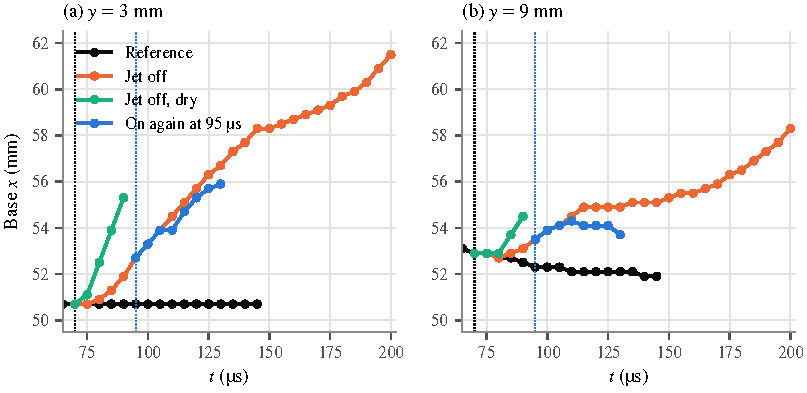
\includegraphics[width=\linewidth]{figures/fig_off.pdf}
\caption{Base position after the jet is switched off at 70\us\ (left dotted line), at (a) $y$ = 3~mm and (b) $y$ = 9~mm. Jet off: residual liquid left in place, continued to 200\us. Dry: all jet liquid removed at switch-off. On again: jet restored at 95\us\ (right dotted line). The base holds for about 10\us\ with the residual liquid and retreats at once without it.}\label{fig:off}
\end{figure}

\begin{figure}[tbp]
\centering
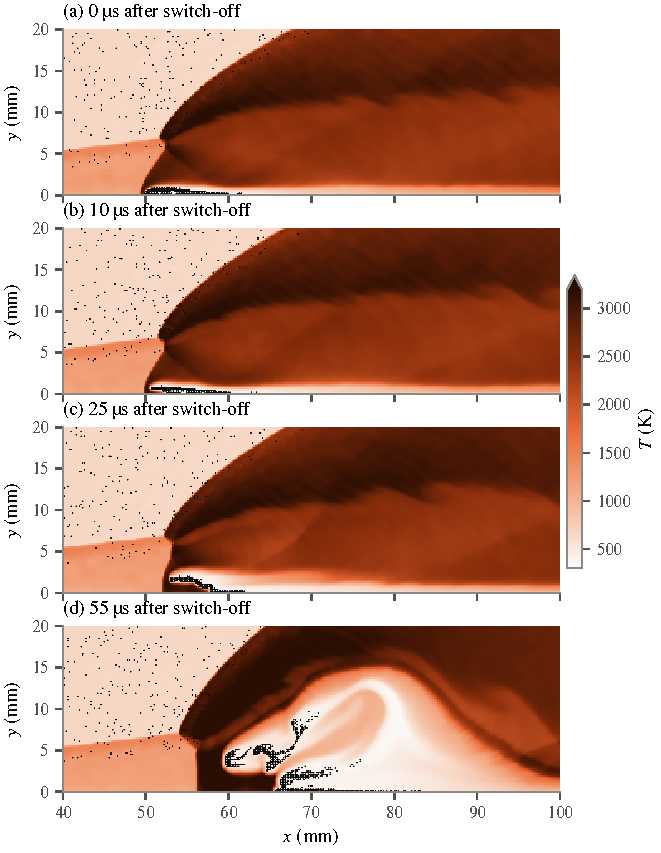
\includegraphics[width=\linewidth]{figures/fig_offsnap.pdf}
\caption{Near-jet temperature and droplets (dots) at (a) 0, (b) 10, (c) 25 and (d) 55\us\ after the jet is switched off at 70\us. The liquid layer persists through (b) and (c) and has moved downstream and broken up by (d).}\label{fig:offsnap}
\end{figure}

Figure~\ref{fig:mechanism} summarizes this sequence. While the liquid layer stays at the jet, the base holds; once the layer slides downstream, the base goes with it, and when the jet returns the base continues to retreat until a new jet-induced OSW has rebuilt from the wall upward. Section~\ref{sec:model} tests how far the hold time $\tau \approx$ 10\us\ and the retreat speed $v_r \approx$ 0.12--0.13~mm/\textmu s account for the response to a pulsed jet.

\subsection{Pulsed injection}\label{sec:pulsed}

Figure~\ref{fig:pulsed} shows the base position at $y$ = 3~mm for the three pulsed jets at 50\% duty. At 80~kHz the off-time (6.25\us) is shorter than the hold time, and the base stays 0.4--0.8~mm behind the reference at every save from 95 to 145\us, with no oscillation at the pulse period resolved by the 5\us\ saves. At $y$ = 6--9~mm it stays 0.4--1.4~mm behind.

At 40~kHz the off-time (12.5\us) slightly exceeds the hold time. The base oscillates with the 25\us\ pulse period, about 3~mm peak to peak, between $x$ = 51.5 and 54.5~mm, while the reference holds 50.7~mm. The oscillation lags the pulses by 10--20\us: the retreat that begins late in an off-phase continues into the next on-phase, and the base returns during the following off-phase. The upstream extreme repeats exactly over the second and third cycles (51.5~mm at 120 and 145\us), whereas the downstream extreme moves 0.6~mm further downstream in the third (53.9 to 54.5~mm). At $y$ = 9~mm the front stays at $x$ = 53.5--54.1~mm, 1.3--2.0~mm behind the reference, with no drift over these cycles. Whether the oscillation is bounded or a slow drift is not settled by three cycles.

At 20~kHz the off-time (25\us) is 2.5 times the hold time. The base holds for 10\us\ after the jet stops at 95\us\ and then retreats at about 0.1~mm/\textmu s. When the jet returns at 120\us, the base continues to retreat through the whole 25\us\ on-phase, more slowly over 130--140\us, and stands 3.8~mm behind the reference at 145\us, with the shock at $y$ = 3~mm weakened to a pressure ratio of 3.0 against 6.8 in the reference. Above $y$ = 9~mm the front stays with the reference throughout. Unlike at 40~kHz, the base did not begin to return within the on-phase. With one cycle simulated, it is not known whether a second cycle would oscillate about a displaced position or move the base further downstream.

\begin{figure}[tbp]
\centering
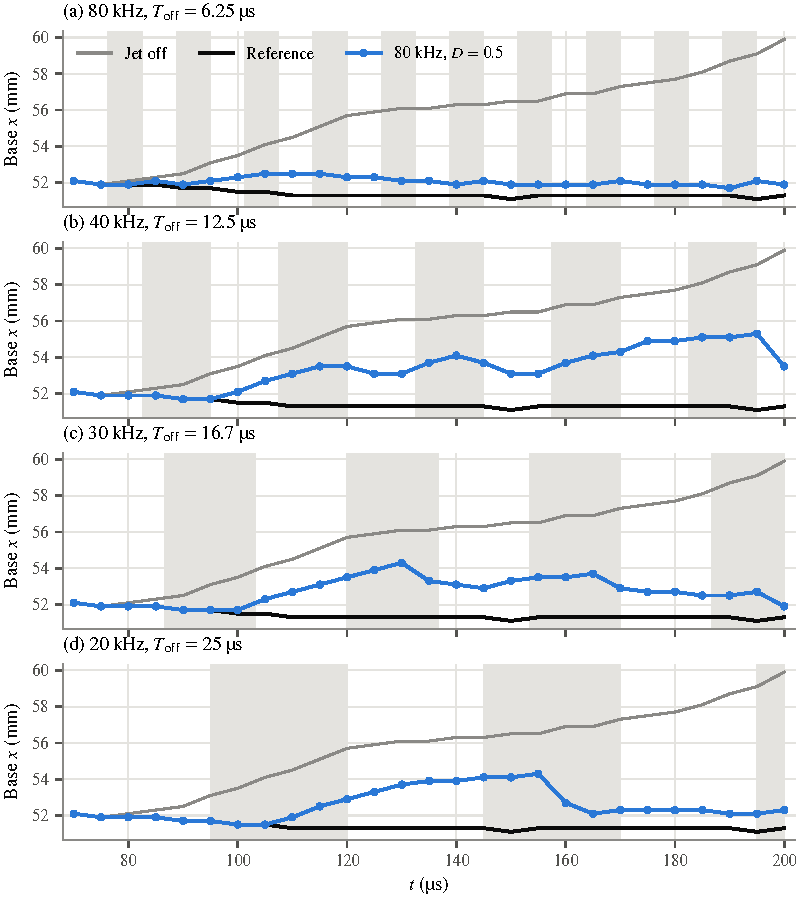
\includegraphics[width=\linewidth]{figures/fig_pulsed.pdf}
\caption{Base position at $y$ = 3~mm under pulsed injection at 50\% duty: (a) 80~kHz, (b) 40~kHz, (c) 20~kHz. Shaded bands mark jet-off phases. Black: reference (continuous jet); grey: jet off.}\label{fig:pulsed}
\end{figure}

\subsection{A hold--retreat--lag model and the critical frequency}\label{sec:model}

The interruption results suggest a simple estimate. If the base holds for $\tau$ after each switch-off and the hold is offset by an equal lag after each switch-on, the excursion per cycle is
\begin{equation}
\Delta x \approx v_r\, T_\mathrm{off} = v_r\,\frac{1-D}{f}, \label{eq:excursion}
\end{equation}
and for $T_\mathrm{off} < \tau$ the base shows only a small offset. This estimate was written down before the 20~kHz run, with $v_r$ = 0.13--0.2~mm/\textmu s, giving 3.3--5~mm. The upper part of that range came from the base at $y$ = 1~mm, which the diagnostic used here no longer tracks (Section~\ref{sec:method}). With the retreat speed at $y$ = 3~mm, 0.12--0.13~mm/\textmu s, Eq.~(\ref{eq:excursion}) gives 1.5--1.6~mm at 40~kHz and 3.0--3.3~mm at 20~kHz (Table~\ref{tab:model}). Measured as the range of base positions over 95--145\us, the simulations give 3.4~mm at 40~kHz (3.0~mm peak to peak over the second and third cycles) and 3.8~mm at 20~kHz, still growing at the end of the run (Fig.~\ref{fig:excursion}). The estimate has the right order and trend but is low by a factor of 1.2--2.3, because the lag after switch-on exceeds the hold after switch-off. After the 12.5\us\ off-phases at 40~kHz the base kept retreating for 10--20\us\ after the jet returned. After a 25\us\ interruption it kept retreating through the whole 25\us\ on-phase at 20~kHz and for at least 15\us\ in the switch-on test of Section~\ref{sec:off}. The lag grows with the distance the base has retreated, which Eq.~(\ref{eq:excursion}) does not represent.

\begin{table}[tbp]
\centering
\small
\caption{Base excursion at $y$ = 3~mm: Eq.~(\ref{eq:excursion}) with $v_r$ = 0.12--0.13~mm/\textmu s, against simulation, as the range of base positions over 95--145\us. Returns: whether the base moves back upstream within an on-phase. The 25\% duty case is in the crop. The pre-run estimate for 20~kHz used $v_r$ = 0.13--0.2~mm/\textmu s and gave 3.3--5~mm.}\label{tab:model}
\begin{tabular}{@{}lllll@{}}
\toprule
$f$ (kHz), $D$ & $T_\mathrm{off}$ (\textmu s) & Eq.~(\ref{eq:excursion}) & Simulated & Returns\\
\midrule
80, 0.5 & 6.25 ($< \tau$) & small offset & 0.4--0.8~mm offset & --\\
40, 0.5 & 12.5 & 1.5--1.6~mm & 3.4~mm (3.0 in cycles 2--3) & yes\\
20, 0.5 & 25 & 3.0--3.3~mm & 3.8~mm at 145\us, growing & no\\
80, 0.25 & 9.4 ($< \tau$) & small offset & 5.0~mm after 40\us, growing & no\\
\bottomrule
\end{tabular}
\end{table}

\begin{figure}[tbp]
\centering
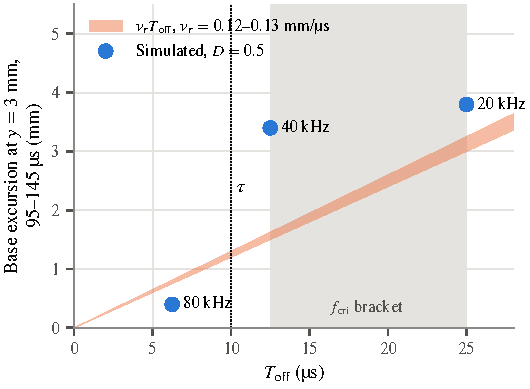
\includegraphics[width=0.62\linewidth]{figures/fig_excursion.pdf}
\caption{Base excursion at $y$ = 3~mm (range of positions over 95--145\us) against the off-time per period at 50\% duty, with the estimate $v_r T_\mathrm{off}$ for $v_r$ = 0.12--0.13~mm/\textmu s. The dotted line marks the hold time $\tau$; the shaded interval is the bracket on $f_\mathrm{cri}$ from the performance results (40--20~kHz).}\label{fig:excursion}
\end{figure}

A minimum frequency follows from requiring $T_\mathrm{off} < \tau$: $f_\mathrm{min} \approx (1-D)/\tau \approx$ 50~kHz at 50\% duty. The performance results of Section~\ref{sec:performance} place the frequency at which pulsing stops matching the continuous jet lower, between 20 and 40~kHz, because short excursions beyond $\tau$ recover within the next on-phase before they cost performance. We call this frequency $f_\mathrm{cri}$, by analogy with Jiang et al. \cite{Jiang2025energy}, who found 8.5--25.6~kHz for pulsed energy deposition on a wedge in a premixed hydrogen--air mixture at Mach~7, decreasing with pulse energy. The two are not the same quantity. Their $f_\mathrm{cri}$ is set by the time for the detonation from one pulse to meet the next before the end of the wedge, because each pulse initiates a new wave. Here the detonation persists through the off-phase, and $f_\mathrm{cri}$ is set by how long the front base stays anchored without the jet. Our bracket rests on one cycle at 20~kHz and three at 40~kHz in single realizations, so it should be read as indicative rather than as a resolved boundary.

The hold time is close to the time the jet takes to inject one jet width of liquid, $d_j/u_j$ = 0.5~mm / 60.83~m/s = 8.2\us, which suggested that $\tau$ might scale with $d_j/u_j$ at fixed J. The 1~mm jet tests this (Fig.~\ref{fig:width}). With the jet on, its base sits at $x$ = 49.9~mm at $y$ = 3~mm and 58.3~mm at $y$ = 15~mm, 0.8 and 3.0~mm upstream of the 0.5~mm jet's at the same time. After switch-off the base moves 0.2~mm in the first 10\us, as for the 0.5~mm jet, so the hold time does not double. The retreat that follows is about half as fast: 0.067~mm/\textmu s over 10--25\us\ after switch-off, against 0.12~mm/\textmu s, and after 25\us\ the base has moved 1.2~mm against 2.0~mm (1.4 against 2.6~mm after 30\us, where the 1~mm run ends). The 1~mm jet leaves twice the liquid near the wall (4.3 against 2.2~mg at switch-off), and its layer slides downstream at about half the speed (the 25\% point at 0.08 against 0.13~mm/\textmu s over 10--25\us), with the base again 0.8--1.0~mm upstream of it (Fig.~\ref{fig:edge}). A wider jet slows the retreat but does not lengthen the hold. In Eq.~(\ref{eq:excursion}) this halves the excursion at a given off-time, which suggests that $f_\mathrm{cri}$ falls with jet width, though not as $u_j/d_j$; the per-area momentum flux also differs between the two jets (1.0 against 1.25 times nominal), and only two widths were run, so the dependence is not resolved.

\begin{figure}[tbp]
\centering
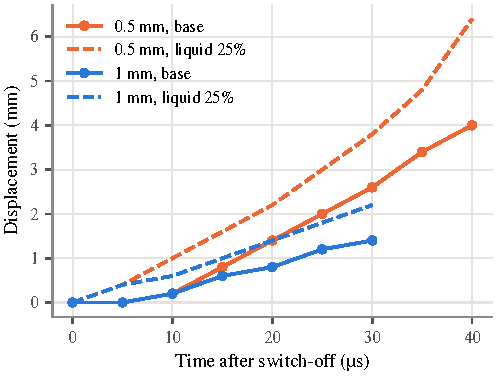
\includegraphics[width=0.62\linewidth]{figures/fig_width.pdf}
\caption{Effect of jet width on the response to switch-off at J = 1 in the crop: displacement of the base at $y$ = 3~mm (solid) and of the 25\% mass point of the wall liquid layer (dashed) since switch-off at 50\us, for the 0.5 and 1~mm jets. Both hold for about 10\us; the 1~mm jet's layer and base then move at about half the speed.}\label{fig:width}
\end{figure}

\subsection{Pulses shorter than the hold: 25\% duty}\label{sec:duty}

At 80~kHz and 25\% duty the jet is on for 3.1\us\ and off for 9.4\us\ per period, so each off-time is shorter than $\tau$. If the hold depended only on the off-time, the base would be held as at 80~kHz and 50\% duty. Instead, over 40\us\ in the crop (Fig.~\ref{fig:edge}(b)), the base at $y$ = 3~mm retreats as with the jet off, from $x$ = 50.7 to 53.5~mm at 30\us, and ends 1.0~mm further downstream than the jet-off base (55.7 against 54.7~mm at 40\us). Near the wall the reaction separates from the shock: at $y$ = 1~mm the gap between the shock and burnt gas grows from 7.2~mm at 25\us\ to 13.6~mm at 40\us, and at $y$ = 3~mm it reaches 13.6~mm at 40\us, with the shock pressure ratio there down to 3.5. At $y$ = 9--15~mm the front stays within 1.6~mm of the jet-off case.

The liquid layer shows why (Fig.~\ref{fig:edge}(b)). The short pulses keep a little liquid at the jet, so that the 5\% mass point stays at $x$ = 50.5--51.9~mm, and the layer as a whole holds more liquid than with the jet off (2.3--2.5 against 1.4--2.3~mg). The bulk of the layer nevertheless slides downstream at 0.14~mm/\textmu s, as with the jet off, and the base stays within 0.6~mm upstream of its 25\% point. Each 3.1\us\ pulse adds too little liquid to stop the layer from being dragged away. A pulsed jet therefore holds the base only when both conditions are met: the off-time must be short compared with the time the layer takes to move, and each on-phase must deliver enough liquid to keep the layer in place. The second condition sets a minimum duty, which lies between 25 and 50\% at 80~kHz for this jet. The extra separation of the reaction near the wall, which the jet-off case does not show, is consistent with the cold liquid of each pulse cooling the near-wall gas without restoring the jet-induced OSW, but no run isolates it.

\subsection{Performance}\label{sec:performance}

Table~\ref{tab:performance} and Fig.~\ref{fig:performance} give the total-pressure recovery and burnt fuel on the measurement plane. In the continuous-jet case the stream processed by the jet loses about 88\% of its total pressure by $x$ = 100~mm, and most of this loss occurs at the detonation itself rather than at the jet.

\begin{table}[tbp]
\centering
\small
\caption{Performance on the plane $x$ = 100~mm, $y <$ 25~mm, averaged over the saves in each window (five; three for the jet-off case), each against the reference over the same window. The noise floor is $\pm$0.002 in recovery and $\pm$0.04~g/s in burnt fuel.}\label{tab:performance}
\begin{tabular}{@{}lllllll@{}}
\toprule
Case & Jet fuel & Window (\textmu s) & \multicolumn{2}{l}{Recovery} & \multicolumn{2}{l}{Burnt fuel (g/s)}\\
 & & & case & ref. & case & ref.\\
\midrule
80~kHz, $D$ = 0.5 & 50\% & 125--145 & 0.116 & 0.116 & 2.41 & 2.37\\
40~kHz, $D$ = 0.5 & 50\% & 125--145 & 0.116 & 0.116 & 2.41 & 2.37\\
20~kHz, $D$ = 0.5 & 50\% & 125--145 & 0.107 & 0.116 & 2.32 & 2.37\\
Half width & 50\% & 125--145 & 0.123 & 0.116 & 2.44 & 2.37\\
Half velocity & 50\% & 125--145 & 0.137 & 0.116 & 2.48 & 2.37\\
Jet off & 0 & 120--130 & 0.082 & 0.118 & 2.10 & 2.38\\
\bottomrule
\end{tabular}
\end{table}

At 80 and 40~kHz the pulsed jets match the reference within the noise floor in both quantities with half the jet fuel, but do not exceed it. At 20~kHz recovery is 8\% below the reference, four times the noise floor, and burnt fuel is 0.05~g/s lower, which is within the noise. Without the jet, recovery is 30\% below the reference 50--60\us\ after switch-off. The ordering of the cases is the same on the planes $y <$ 20 and $y <$ 30~mm and at $x$ = 110~mm. Within the 40~kHz window, the last save (145\us) alone is low, 0.104 against 0.113; it coincides with the 0.6~mm growth of the downstream excursion noted in Section~\ref{sec:pulsed}, and the five-save average still matches the reference.

Resolving the recovery by height locates the losses (Fig.~\ref{fig:performance}(b)). Above $y$ = 15~mm all cases agree within 0.002. Without the jet the loss lies at $y$ = 3--15~mm, and 6~g/s less mass crosses the plane below $y$ = 25~mm, so the flow there is displaced away from the wall. At 125\us\ the subsonic wall region left by the decaying pocket spans $x$ = 65.5--95.1~mm, just upstream of the plane, which suggests that the jet-off loss comes from this region approaching the plane rather than from the retreat of the base itself. If so, it is a transient. The continued jet-off run could not settle this: after 130\us, cold fuel-rich gas from the pocket crosses the plane, the mass flux through it swings between 28 and 91~g/s, and the metric is no longer usable there.

\begin{figure}[tbp]
\centering
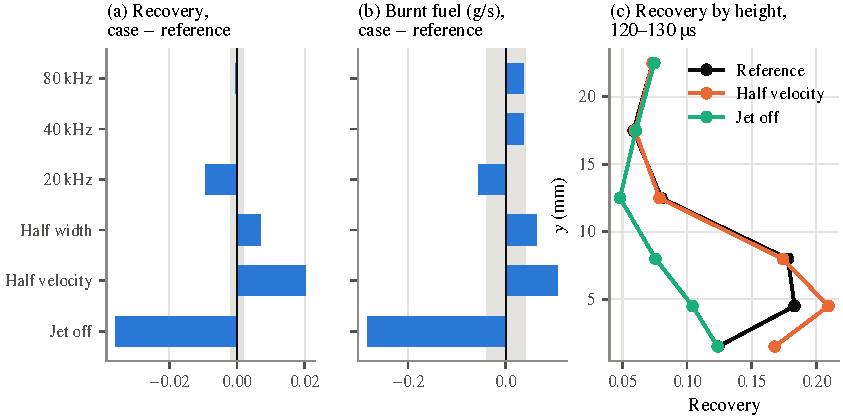
\includegraphics[width=\linewidth]{figures/fig_performance.pdf}
\caption{Performance on the plane $x$ = 100~mm, $y <$ 25~mm. (a) Total-pressure recovery and (b) burnt fuel, as the case minus the reference over the same window (125--145\us; jet off 120--130\us); the shaded band is the noise floor. (c) Recovery by height band, averaged over 120--130\us, for the reference, the half-velocity jet and the jet-off case.}\label{fig:performance}
\end{figure}

\subsection{Pulsed and steady jets at equal fuel}\label{sec:equalfuel}

A 50\% pulse at J = 1 delivers half the fuel of the continuous jet. A steady jet can deliver the same mean fuel in two ways: at half the velocity, which lowers J to 0.25, or at half the width, which keeps J = 1. Figure~\ref{fig:equalfuel} compares both with the pulsed jets.

Over the first 75\us\ the half-velocity jet holds the base no better than no jet. By 145\us\ the base at $y$ = 3~mm is 7.4~mm behind the reference ($x$ = 58.1 against 58.3~mm with the jet off) and retreating at about 0.1~mm/\textmu s. Continued to 200\us, however, the two separate. The half-velocity base slows from 0.08~mm/\textmu s over 145--160\us\ to 0.02~mm/\textmu s over 190--200\us\ and settles near $x \approx$ 61~mm, about 10~mm behind the reference, with its shock at $y$ = 3~mm weakened to a pressure ratio of 3.4. Over the same interval the jet-off base speeds up from 0.03 to 0.12~mm/\textmu s. It does not revert to the mode that Ref.~\cite{Wang2026ast} finds from a cold start below J = 0.4, in which the jet only enriches the mixture and the ODW initiates about 80~mm downstream. The front formed at J = 1 thus stays anchored at a J that does not anchor a front from a cold start. The same history dependence appears without any jet, where the spray never ignites from a cold start (Section~\ref{sec:validation}) but an anchored front survives 130\us\ after the jet stops (Section~\ref{sec:off}). Its recovery is nevertheless the highest of all cases, 0.137 against 0.116, with slightly more burnt fuel (2.48 against 2.37~g/s). The gain lies entirely in the lowest 6~mm (Fig.~\ref{fig:performance}(b)), where the near-wall stream passes a weaker jet shock. A retreating base does not by itself lower recovery on this plane, which supports the reading above that the jet-off loss comes from the displaced wall flow.

The half-width jet holds the base within 0.8~mm of the reference at $y$ = 3~mm up to 120\us, as the 80~kHz pulse does, and its recovery over 125--145\us\ is 0.123, at least the reference's. Its base then creeps downstream at about 0.06~mm/\textmu s, at $y$ = 2--4~mm alike, and stands 2.2~mm behind the reference at 145\us\ ($x$ = 52.9~mm), when the run ends, whereas the 80~kHz base stays 0.4--0.8~mm behind. Whether the narrow jet's base settles was not determined. Two caveats apply. The half-width jet is a single cell wide and is injected by a cone injector on that cell, and a narrower slot in two dimensions is not equivalent to a smaller round jet in three.

Together, the two steady jets separate the roles of momentum and fuel. The base stays at the jet when J is above the direct-initiation threshold while the jet is on, not when a given mean fuel flow is supplied; a pulse keeps J at its full value during each on-phase, and the liquid layer bridges off-phases shorter than about $\tau$, provided each on-phase replenishes it (Section~\ref{sec:duty}). In this configuration, at 50\% fuel, pulsing therefore offers no advantage in recovery or burnt fuel over a correctly sized steady jet over the 75\us\ simulated, although the steady jet's base was drifting at the end. With a fixed injector, however, the narrower jet is not available: the fuel flow can be cut only by throttling, which lowers J as the square of the fuel fraction, or by pulsing. At 50\% fuel, pulsing at 80~kHz keeps the base within 0.8~mm of the reference, while throttling lets it settle about 10~mm downstream; both keep an anchored front. Throttling keeps J above 0.4 only down to 63\% of the full jet fuel, and at 25\% fuel a throttled jet would be at J = 0.06, below every case of Ref.~\cite{Wang2026ast}; pulsing at 80~kHz holds the base at 50\% fuel but not at 25\% (Section~\ref{sec:duty}). For a fixed injector, pulsing thus extends the range of fuel flow over which the base stays at the jet, to a limit between 25 and 50\% of the full jet fuel at this frequency.

\begin{figure}[tbp]
\centering
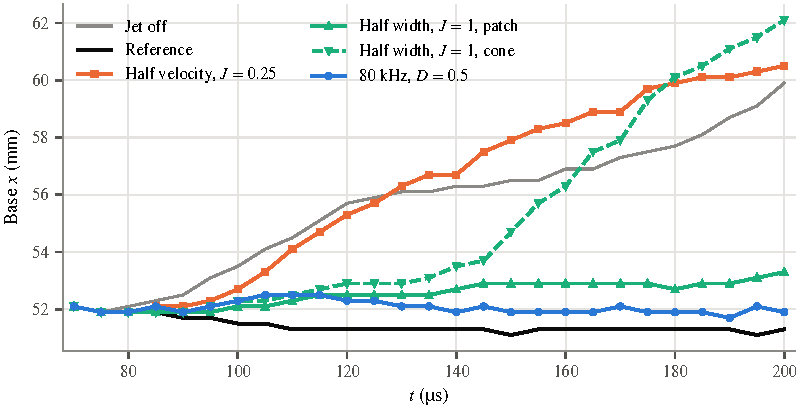
\includegraphics[width=\linewidth]{figures/fig_equalfuel.pdf}
\caption{Base position at $y$ = 3~mm for jets delivering 50\% of the continuous-jet fuel, with the reference and the jet-off case; the 40~kHz pulse is shown in Fig.~\ref{fig:pulsed}(b). The steady jet at the same J (half width) holds the base as the 80~kHz pulse does up to 120\us\ and then drifts downstream; the steady jet at J = 0.25 (half velocity) follows the jet-off case to 145\us\ and then settles about 10~mm downstream, while the jet-off base keeps retreating.}\label{fig:equalfuel}
\end{figure}

\subsection{Comparison with forced steady-jet anchoring}

Wang et al. \cite{Wang2026confined} forced the inlet pressure of a confined combustor while holding the jet steady, and found bounded triple-point excursions of up to 3--5~mm at a forcing amplitude of 0.5 and 4~kHz, lost only when J was too large. In the present case the flow is steady and the jet is forced. The two have in common a finite response time of the coupled shock, droplet and reaction system, which in both makes the wave lag the forcing. Here the response time can be measured directly as the hold time and the recovery lag. The excursions at 20 and 40~kHz (2--4~mm) are of the same order as theirs, at five to ten times their forcing frequency, for a 0.5~mm jet against their 10~mm jet. Whether the two response times are related through $d_j/u_j$ cannot be checked from the published data, and the comparison is one of order only. The sweeping jet of Fan et al. \cite{Fan2024sweeping} differs in kind: its gaseous jet is never off, and it is redirected rather than interrupted, so it has no counterpart to the residual-liquid hold found here.

\begin{figure}[tbp]
\centering
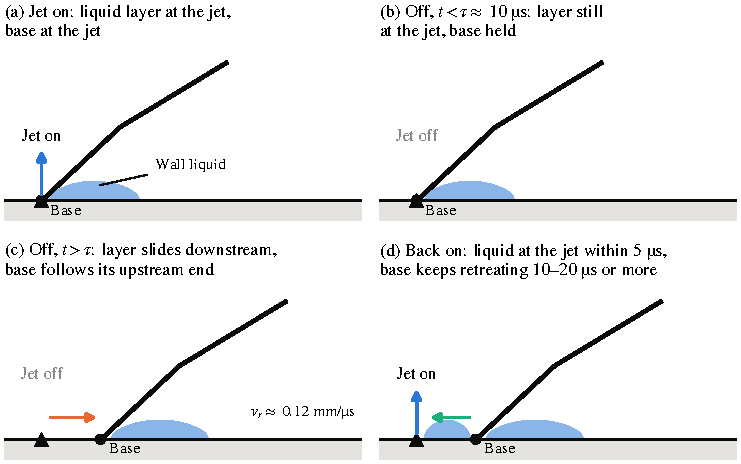
\includegraphics[width=\linewidth]{figures/fig_mechanism.pdf}
\caption{Schematic of the base response to jet interruption (not to scale). (a) Jet on: the liquid the jet leaves on the wall lies at the jet, and the base sits at the jet. (b) Jet off, $t < \tau$: the layer is still at the jet and the base holds. (c) Jet off, $t > \tau$: the layer slides downstream without losing mass, and the base follows its upstream end at $v_r$. (d) Jet back on: liquid is again at the jet within 5\us, but the base keeps retreating for 10--20\us\ after a 12.5\us\ interruption, and longer after a longer one. Values are from Sections~\ref{sec:off} and \ref{sec:pulsed} and Fig.~\ref{fig:edge}.}\label{fig:mechanism}
\end{figure}

\section{Conclusions}\label{sec:conclusions}

The response of a liquid n-heptane ODW anchored by a transverse liquid n-heptane jet at J = 1 to switching off, switching back on, pulsing and throttling of the jet was computed with a two-dimensional Eulerian--Lagrangian method, after the steady-jet case of Ref.~\cite{Wang2026ast} was reproduced. The main conclusions are as follows.

(1) The jet-anchored ODW does not fail when the jet stops; it still stood 130\us\ after switch-off. Its base holds position for $\tau \approx$ 10\us, then retreats downstream at about 0.12~mm/\textmu s and does not settle within 130\us, while the front above $y$ = 9~mm barely moves. These values agree within 0.1~mm in base position between grids of 0.2 and 0.15~mm over 40\us.

(2) The base is held by the liquid the jet leaves on the wall, and it follows where that liquid is; the liquid mass barely changes. The liquid forms a cold (about 400~K), fuel-rich layer that loses less than 2\% of its mass to evaporation in 20\us. After switch-off it slides downstream at about 0.13--0.14~mm/\textmu s, and the base stays within 1~mm upstream of its 25\% mass point for 25\us. With the jet liquid removed at switch-off, the base retreats 2.3 times sooner.

(3) A 1~mm jet at J = 1 leaves twice the liquid. Its base holds for the same 10\us\ but then retreats at about half the speed (0.067 against 0.12~mm/\textmu s), as its layer does. A wider jet slows the retreat but does not lengthen the hold.

(4) When the jet returns, the liquid re-forms at the jet within 5\us, but the base keeps retreating: for 10--20\us\ after a 12.5\us\ interruption, and for more than 25\us\ after a 25\us\ one. Recovery is slower than retreat, and the lag grows with the retreat.

(5) Under pulsing at 50\% duty, the base is held within 0.8~mm at 80~kHz ($T_\mathrm{off} < \tau$), oscillates about 3~mm peak to peak with a 10--20\us\ lag at 40~kHz, and retreats 3.8~mm without recovering within one cycle at 20~kHz. The estimate $v_r(1-D)/f$ gives the order of these excursions but underestimates them by a factor of 1.2--2.3, because of the recovery lag. Total-pressure recovery and burnt fuel stay at the continuous-jet level at 40 and 80~kHz with half the jet fuel, and recovery falls by 8\% at 20~kHz, so the critical frequency for this jet at 50\% duty lies between 20 and 40~kHz.

(6) At 25\% duty and 80~kHz the base retreats as without a jet, although each off-time (9.4\us) is shorter than $\tau$: each 3.1\us\ pulse adds too little liquid to keep the layer at the jet. Holding the base requires a minimum duty as well as a minimum frequency; at 80~kHz it lies between 25 and 50\%.

(7) At the same mean fuel, a steady jet of half the width at J = 1 matches the pulsed jets in recovery and burnt fuel and holds the base within 0.8~mm for 50\us, but its base then drifts to 2.2~mm behind by the end of the run. In this configuration pulsing offers no performance advantage over a steady jet sized to the same J within the time simulated. With a fixed injector, throttling to 50\% fuel (J = 0.25) lets the base settle about 10~mm downstream, whereas pulsing at 80~kHz keeps it within 0.8~mm. The throttled front stays anchored and does not revert to the downstream initiation found from a cold start at that J.

These conclusions are limited in four ways, each of which identifies a specific extension. First, and most important, the liquid layer that holds the base occupies about 30\% of the volume of the wall cells that contain it, far beyond the dilute limit of the point-particle spray model, and its wall interaction is a modelling choice that Ref.~\cite{Wang2026ast} does not specify. Since the base follows the motion of this layer, the hold time and retreat speed are the least certain quantities in this study; a wall-film model with film drag and breakup is needed to test them. Second, the simulations are two-dimensional with a slip wall and no turbulence model, so the drag on the layer and mixing into it are only what the grid resolves; three-dimensional simulations of a round jet are needed to confirm $\tau$ and $v_r$. Third, the frequency and duty brackets rest on one cycle at 20~kHz, three at 40~kHz and three at 25\% duty in single realizations, with no measure of run-to-run scatter; runs at 30~kHz and at 35\% duty would narrow them. Fourth, only two jet widths were run, at slightly different momentum fluxes per unit area; widths of 2 and 4~mm at a common flux would establish how $v_r$, and with it $f_\mathrm{cri}$, depends on jet size.

\section*{CRediT authorship contribution statement}
\textbf{Yuvan Senthilkumar:} Conceptualization, Methodology, Software, Validation, Formal analysis, Investigation, Resources, Data curation, Writing -- original draft, Writing -- review \& editing, Visualization, Project administration, Funding acquisition.

\section*{Declaration of competing interest}
The authors declare that they have no known competing financial interests or personal relationships that could have appeared to influence the work reported in this paper.

\section*{Acknowledgments}
The author thanks Huangwei Zhang (National University of Singapore) and Tsingyoung Meng (The Hong Kong Polytechnic University) for providing the 44-species n-heptane reaction mechanism files. This work received no external funding; it was funded by the author. The simulations were run on a rented Amazon Web Services EC2 c7a.4xlarge instance (16 vCPUs, 32~GiB memory, 200~GB storage).

\section*{Declaration of generative AI and AI-assisted technologies in the writing process}
During the preparation of this work the author used Claude (Anthropic) to write and check parts of the simulation set-up, analysis and plotting code, to manage the cloud computing runs, and to review and revise the author's draft of the text, including its structure. The author directed the study, chose the cases and their interpretation, reviewed and edited all code and text, and takes full responsibility for the content of the publication.

\section*{Data availability}
The case generator, run scripts and analysis tools used for every result in this paper are openly available at \url{https://github.com/Youwes09/pulswave}, together with the solver commit (detonationFoam, two-phase branch, commit 02ed90db0a17, on OpenFOAM-8 commit a86b07b9dabb). Field data are available from the authors on request.

\begin{thebibliography}{99}

\bibitem{Kailasanath2000} K. Kailasanath, Review of propulsion applications of detonation waves, AIAA J. 38 (2000) 1698--1708.

\bibitem{Jiang2023review} Z. Jiang, Standing oblique detonation for hypersonic propulsion: A review, Prog. Aerosp. Sci. 143 (2023) 100955.

\bibitem{Rosato2021} D.A. Rosato, M. Thornton, J. Sosa, C. Bachman, G.B. Goodwin, K.A. Ahmed, Stabilized detonation for hypersonic propulsion, Proc. Natl. Acad. Sci. 118 (2021) e2102244118.

\bibitem{Zhang2022exp} Z. Zhang, C. Wen, C. Yuan, Y. Liu, G. Han, C. Wang, Z. Jiang, An experimental study of formation of stabilized oblique detonation waves in a combustor, Combust. Flame 237 (2022) 111868.

\bibitem{Han2023trip} X. Han, Y. Liu, Z. Zhang, W. Zhang, C. Yuan, G. Han, Z. Jiang, Experimental demonstration of forced initiation of kerosene oblique detonation by an on-wedge trip in an ODE model, Combust. Flame 258 (2023) 113102.

\bibitem{ZhangWen2025} Z. Zhang, C.-Y. Wen, Oblique detonation engines: initiation and stabilization of oblique detonation waves in confined space, Acta Aerodyn. Sin. 43 (9) (2025) 65--91 (in Chinese).

\bibitem{Qin2018modified} Q. Qin, X. Zhang, A novel method for trigger location control of the oblique detonation wave by a modified wedge, Combust. Flame 197 (2018) 65--77.

\bibitem{Liu2026bump} Y. Liu, Numerical investigation of Mach 10 kerosene-fueled oblique detonation waves at different flight altitudes, arXiv:2609.02515 (2026).

\bibitem{Sun2023unsteady} J. Sun, P. Yang, B. Tian, Z. Chen, Evolution and control of oblique detonation wave structure in unsteady inflow, AIAA J. 61 (2023) 4808--4820.

\bibitem{Xin2024laser} Y. Xin, J. Shang, G. Xiang, Q. Wang, Investigation on accelerated initiation of oblique detonation wave induced by laser-heating hot-spot, Aerospace (2024).

\bibitem{Jiang2025energy} Z. Jiang, Z. Chen, L. Shi, Z. Zhang, J. Hao, C.-Y. Wen, Numerical study of oblique detonation initiation assisted by local energy deposition, arXiv:2508.08943 (2025).

\bibitem{Wang2022hotjet} A. Wang, J. Bian, H. Teng, Numerical study on initiation of oblique detonation wave by hot jet, Appl. Therm. Eng. 213 (2022) 118679.

\bibitem{Li2020hotjet} H. Li, J. Li, C. Xiong, W. Fan, L. Zhao, W. Han, Investigation of hot jet on active control of oblique detonation waves, Chin. J. Aeronaut. 33 (2020) 861--869.

\bibitem{Qin2020coflow} Q. Qin, X. Zhang, Study on the initiation characteristics of the oblique detonation wave by a co-flow hot jet, Acta Astronaut. 177 (2020) 86--95.

\bibitem{Han2024jet} X. Han, R. Qiu, Y. You, Flow characteristics and propulsive performance of oblique detonation waves induced by a transverse jet, Phys. Fluids 36 (2024).

\bibitem{ZhangJiang2023jet} Z. Zhang, Z. Jiang, Numerical investigation of transverse-jet-assisted initiation of oblique detonation waves in a combustor, Aerospace 10 (2023) 1033.

\bibitem{Yao2023jetwedge} J. Yao, Z. Lin, Numerical investigation of jet-wedge combinatorial initiation for oblique detonation wave in supersonic premixed mixture, Phys. Fluids 35 (2023).

\bibitem{Fan2024sweeping} J. Fan, Y. Zhang, G. Xiang, Y. Feng, Numerical investigation of sweeping jet actuator on oblique detonation, Combust. Flame 268 (2024) 113622.

\bibitem{Ren2018jfm} Z. Ren, B. Wang, G. Xiang, L. Zheng, Effect of the multiphase composition in a premixed fuel--air stream on wedge-induced oblique detonation stabilisation, J. Fluid Mech. 846 (2018) 411--427.

\bibitem{Ren2019pci} Z. Ren, B. Wang, G. Xiang, L. Zheng, Numerical analysis of wedge-induced oblique detonations in two-phase kerosene--air mixtures, Proc. Combust. Inst. 37 (2019) 3627--3635.

\bibitem{Teng2023droplet} H. Teng, C. Tian, P. Yang, M. Zhao, Effect of droplet diameter on oblique detonations with partially pre-vaporized n-heptane sprays, Combust. Flame 258 (2023) 113062.

\bibitem{Tian2024jfm} C. Tian, H. Teng, B. Shi, P. Yang, K. Wang, M. Zhao, Propagation instabilities of the oblique detonation wave in partially prevaporized n-heptane sprays, J. Fluid Mech. 984 (2024) A16.

\bibitem{Wang2025cnf} W. Wang, Z. Hu, P. Zhang, Computational investigation on the formation of liquid-fueled oblique detonation waves, Combust. Flame 271 (2025) 113839.

\bibitem{Wang2026ast} W. Wang, Z. Hu, P. Zhang, Liquid-fueled oblique detonation waves induced by reactive and non-reactive transverse liquid jets, Aerosp. Sci. Technol. 168 (2026) 111293.

\bibitem{Wang2026confined} W. Wang, Z. Hu, P. Zhang, Liquid-fueled oblique detonation stabilized by a transverse jet, arXiv:2605.27871 (2026).

\bibitem{Liu2018hysteresis} Y. Liu, L. Wang, B. Xiao, Z. Yan, C. Wang, Hysteresis phenomenon of the oblique detonation wave, Combust. Flame 192 (2018) 170--179.

\bibitem{Liu2004mech} S. Liu, J.C. Hewson, J.H. Chen, H. Pitsch, Effects of strain rate on high-pressure nonpremixed n-heptane autoignition in counterflow, Combust. Flame 137 (2004) 320--339.

\bibitem{Wang2024breakup} W. Wang, M. Yang, Z. Hu, P. Zhang, A dynamic droplet breakup model for Eulerian--Lagrangian simulation of liquid-fueled detonation, Aerosp. Sci. Technol. 151 (2024) 109271.

\bibitem{Pilch1987} M. Pilch, C. Erdman, Use of breakup time data and velocity history data to predict the maximum size of stable fragments for acceleration-induced breakup of a liquid drop, Int. J. Multiphase Flow 13 (1987) 741--757.

\bibitem{Ranz1952} W.E. Ranz, W.R. Marshall, Evaporation from drops, Chem. Eng. Prog. 48 (1952) 141--146.

\bibitem{Crowe1977} C.T. Crowe, M.P. Sharma, D.E. Stock, The particle-source-in cell (PSI-CELL) model for gas-droplet flows, J. Fluids Eng. 99 (1977) 325--332.

\bibitem{Sun2023detonationfoam} J. Sun, Y. Wang, B. Tian, Z. Chen, detonationFoam: An open-source solver for simulation of gaseous detonation based on OpenFOAM, Comput. Phys. Commun. 292 (2023) 108859.

\bibitem{Kurganov2001} A. Kurganov, S. Noelle, G. Petrova, Semidiscrete central-upwind schemes for hyperbolic conservation laws and Hamilton--Jacobi equations, SIAM J. Sci. Comput. 23 (2001) 707--740.

\bibitem{Abramzon1989} B. Abramzon, W.A. Sirignano, Droplet vaporization model for spray combustion calculations, Int. J. Heat Mass Transfer 32 (1989) 1605--1618.

\bibitem{Guo2023pci} H. Guo, Y. Xu, H. Zheng, H. Zhang, Ignition limit and shock-to-detonation transition mode of n-heptane/air mixture in high-speed wedge flows, Proc. Combust. Inst. 39 (2023) 4771--4780.

\end{thebibliography}

\end{document}
